% !Mode:: "TeX:UTF-8"
% !TEX root = ..\proposal.tex

\chapter{采用的关键技术及技术路线}
\section{关键技术}
装配车间调度的关键技术是和调度相关的技术,需要有调度理论的框架和相关概念,常用的调度模型可分为确定型模型和随机型模型,它们的区别是随机型模型的相关变量不是具体值,而是一个分布,不同的情况下用到的分布,包括连续分布和离散的,使模型更接近实际情况。

除了调度的结构体系,其实现算法也相当关键,和本研究的相关算法中,选取3个具有代表的:完整批产品簇排序(FBFS)、变领域搜索(VNS)和粒子群优化算法(PSO)。FBFS 算法的特点是将作业按簇分成批次,可以有效减少作业簇准备时间,适合多品种的生产调度,这是直接从调度本身入手的,可操作性很大,而且较符合实用情况,虽然有其不完善,但改善比较容易。VNS 和PSO 都是解的搜索方法,理论性较强,可以将两者结合实用,比如在VNS 随机下一个领域的的阶段可以通过PSO 来确定下一个搜索方向,发货两者的优势。只是仅从目标函数的解空间搜索,获得的结果可能会在实用中出现相关问题,需要进一步通过实践研究。
\section{技术路线}
本课题采用的基本思路和关键技术路线如\reff{fig:1}所示。
\begin{figure}[h]
\centering
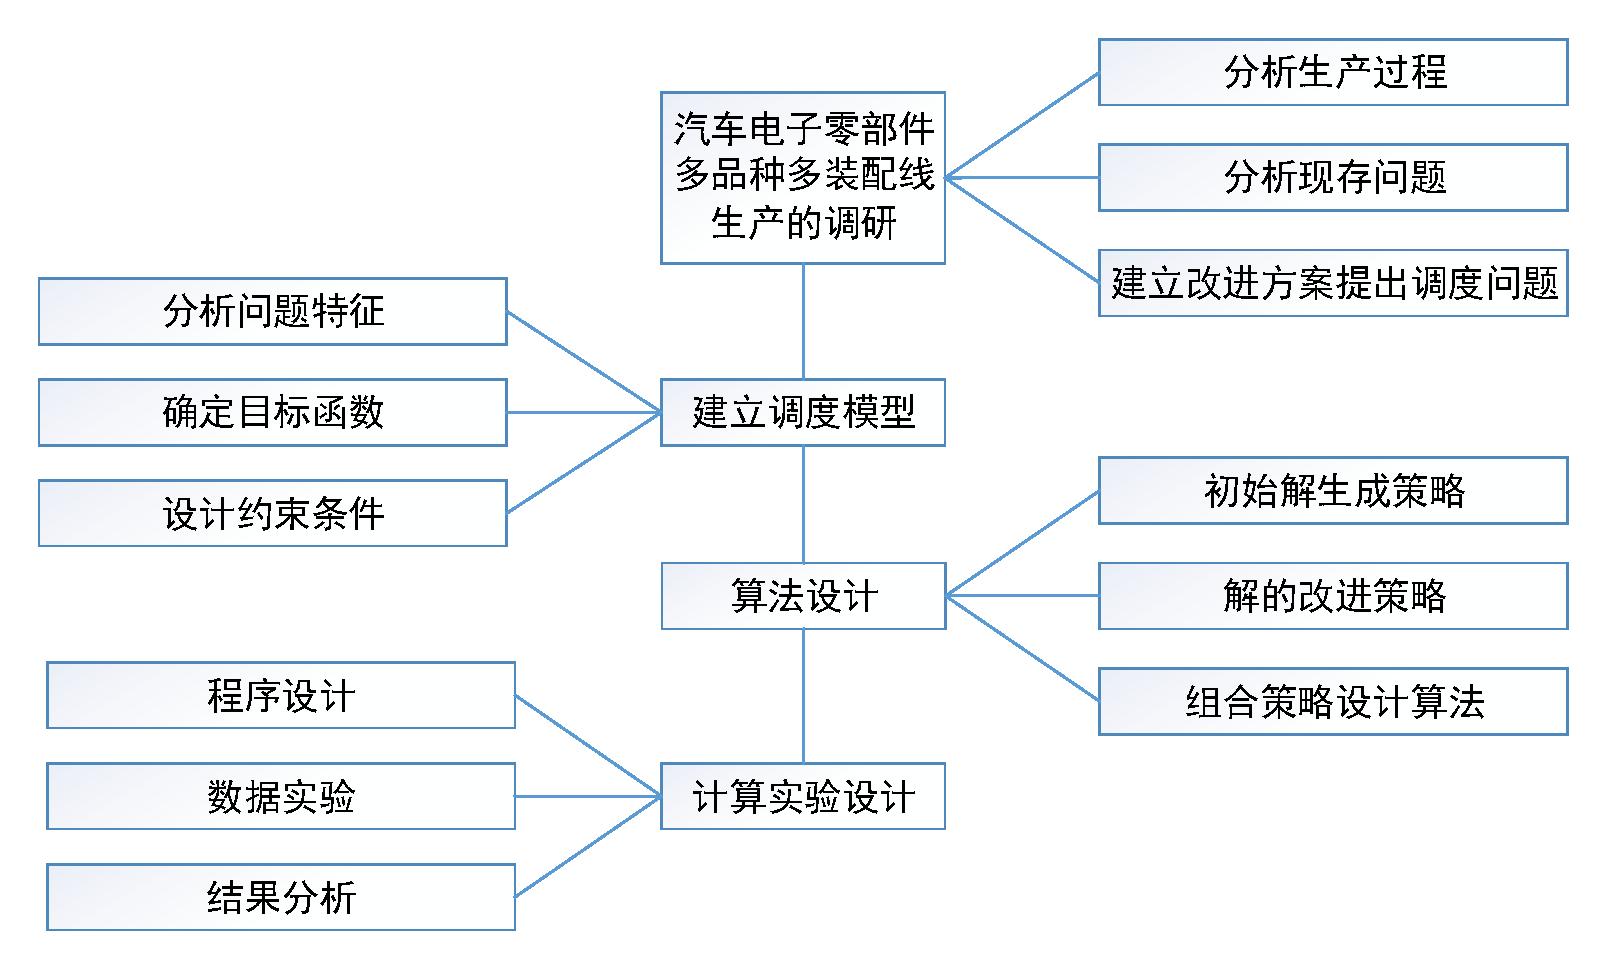
\includegraphics[width = 10cm]{techroute1.pdf}
\caption{基本思路和关键技术路线\label{fig:1}}
\end{figure}